\documentclass{beamer}

\mode<presentation>
{
  \usetheme{Frankfurt}      % or try Darmstadt, Madrid, Warsaw, ...
  %% \usecolortheme{default} % or try albatross, beaver, crane, ...
  \usecolortheme[RGB={0,104,139}]{structure}%deepskyblue
  \usefonttheme{serif}  % or try serif, structurebold, ...
  \setbeamertemplate{navigation symbols}{}
  \setbeamertemplate{caption}[numbered]
  \useinnertheme{rounded}
}

\usepackage{array}
\usepackage{graphicx}
\usepackage{hyperref}
\usepackage{pxfonts}
\usepackage[english]{babel}
\usepackage[utf8x]{inputenc}
\usepackage[font=small,labelfont=bf]{caption}
\usepackage{amsmath}
\usepackage{tikz}
\usetikzlibrary{arrows,shapes}
\setbeamercovered{transparent}
%% 
\title[Sandhi
\insertframenumber/\inserttotalframenumber]{Sandhi\\ Open Source Visual Programming Software}
\author[Sandhi Team, IIT Bombay]{Ambikeshwar Srivastava \\FOSSEE, IIT Bombay \\Manoj Gudi\\ CTO, Focus Analytics}
\date{August 22,2015}
\usepackage{beamerthemesplit}
\usepackage{beamerthemeshadow}
\logo{
\includegraphics[width=1cm height=2cm]{fosseelogo.png}
    \hspace{\dimexpr \paperwidth-2cm-5pt}

\includegraphics[height=1cm]{iitblogo.pdf}}

\begin{document}
\begin{frame}
\titlepage
\end{frame}

\begin{frame}
	\frametitle{Introduction}
	\begin{itemize}
		\item Sandhi is a visual programming editor based on GNU Radio
		\item Basic data structure in sandhi is the flowgraph
		\item It has been named Sandhi as it means connecting and conveys our idea of connecting various blocks to come up with a robust visual program
		\item Sandhi is aimed to become a visual programming tool for replacing LabVIEW
	\end{itemize}
\end{frame}

\begin{frame}
        \frametitle{Flowgraph}
        \begin{itemize}
        \item Flowgraph represents the connections of the blocks through which a continuous stream of samples flows
        \item The concept of a flowgraph is an acyclic directional graph:
	\begin{itemize}
	\item  with one or more source blocks (to insert samples into the flowgraph) 
	\item  one or more sink blocks (to terminate or export samples from the flowgraph) and 
	\item  any functional blocks in between.
	\end {itemize}
        \end{itemize}
	\vspace{-0.14in}
        \begin{figure}
        \centering
        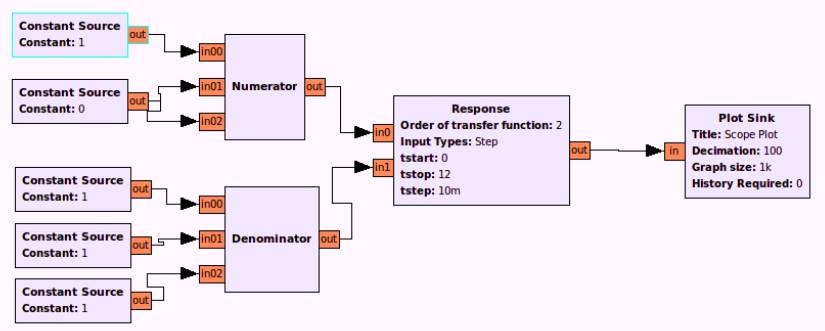
\includegraphics[height=2.8cm, width=10cm]{step_resp.png}
	\caption{Flowgraph}
        \end{figure}
        \vspace{-0.2in}

\end{frame}

\begin{frame}
        \frametitle{Motivation to develop Sandhi}
        \begin{itemize}
		\item  Lack of proper open source alternative to LabVIEW.
		\item  Expensive proprietary software.
		\item  Being FOSS, it gives you freedom to modify, share and sell your application without any permission. 
        \end{itemize}
\end{frame}

\begin{frame}
        \frametitle{Development of Sandhi}
        \begin{itemize}
                \item GNU Radio
                \item sciscipy
                \item GRAS
        \end{itemize}
\end{frame}

\begin{frame}
        \frametitle{GNU Radio}
        \begin{itemize}
		\item GNU Radio is a free and open-source software development toolkit that provides signal processing blocks to implement software radios.
		\item Supposed to be used by the Electrical Engineering community for the purpose of digital signal processing 
		\item It has a rich module of implemented device drivers and thereby supports a range of devices
        \end{itemize}
\end{frame}

\begin{frame}
        \frametitle{Why GNU Radio?}
        \begin{itemize}
                \item GNURadio is a very promising visual programming tool as:
        \begin{itemize}
                \item it make very easy for the developer to abstract his code
                \item provides a very easy to use framework to the developer
                \item it is open source
        \end{itemize}
        \end{itemize}
\end{frame}

\begin{frame}
	\frametitle{sciscipy}
	\begin{itemize}
		\item Sciscipy is an Application Programming Interface 
		\item Aimed for Inter Process Communication with scilab when in workspace of Python programming language
	\end{itemize}
	\textbf{Sample Code:}\\ 
	\textit{from scilab import Scilab 
                \\  sci = Scilab()
                \\  x = sci.rand(20, 20)
                \\  y = x*x.transpose()
                \\  y\_inv = sci.inv(y)}
\end{frame}

\begin{frame}
        \frametitle{GRAS}
        \begin{itemize}
		\item GRAS stands for GNU Radio Advanced Scheduler
		\item It was impossible to implement the feedback with GNU Radio, which uses stock application schedular \newline 
        \end{itemize}
\textit{\textbf{Note:} Application Scheduler is responsible for threading, controlling the data flow and managing the use of the computer resources like processor time to various processes.}

\end{frame}

\begin{frame}
        \frametitle{Blocks in sandhi}
        \begin{itemize}
	\item Blocks are the basic building component of flowgraph
	\item Blocks have the property written in C++ or Python
        \end{itemize}
\begin{figure}
        \centering
        \begin{minipage}{.3\textwidth}
            \centering
            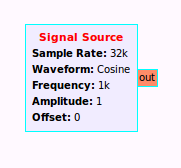
\includegraphics[width=.9\linewidth]{source_block.png}
            \caption{Source}
        \end{minipage}%
        \begin{minipage}{.3\textwidth}
            \centering
            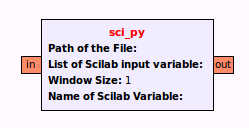
\includegraphics[width=.9\linewidth]{process_block.png}
            \caption{Process}
        \end{minipage}%
	\begin{minipage}{.3\textwidth}
            \centering
            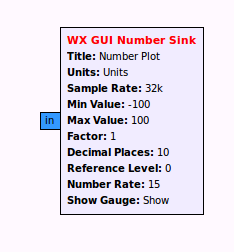
\includegraphics[width=.9\linewidth]{sink_block.png}
            \caption{Sink}
        \end{minipage}
    \end{figure}

\end{frame}

\begin{frame}
	\frametitle{Sandhi GUI}
	\begin{figure}
	\centering
	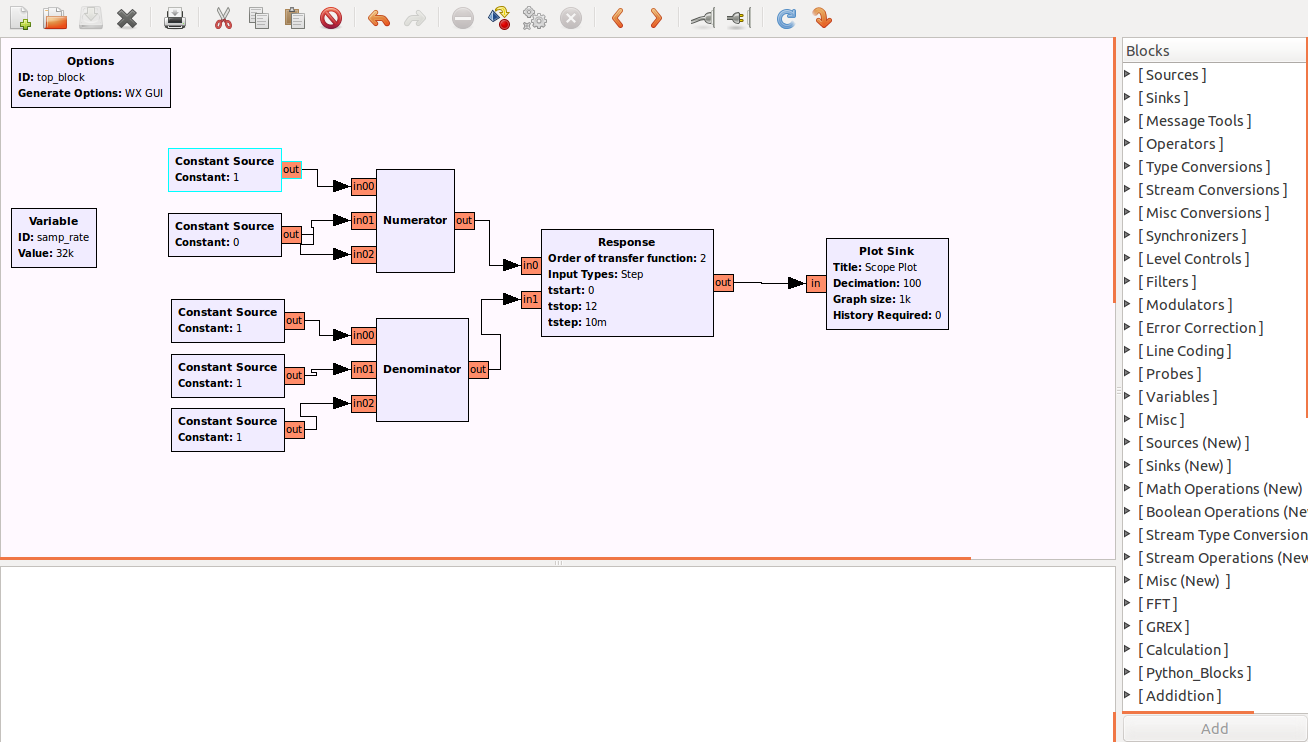
\includegraphics[width=.9\linewidth]{sandhi_GUI.png}
	\caption{Sandhi GUI}
	\end{figure}
\end{frame}

\begin{frame}
        \frametitle{How to create a block}
        \begin{itemize}
        \item One can create a customized block with knowledge of C++ or Python
        \item Block developer have access to any library available in Python
	\item There are two files needed to create a block in sandhi:
		\begin{itemize}
			\item Functionality written in C++ or Python
			\item Properties written in xml file
		\end{itemize}
        \end{itemize}
%\begin{figure}
%        \begin{minipage}{.5\textwidth}
%            \centering
%            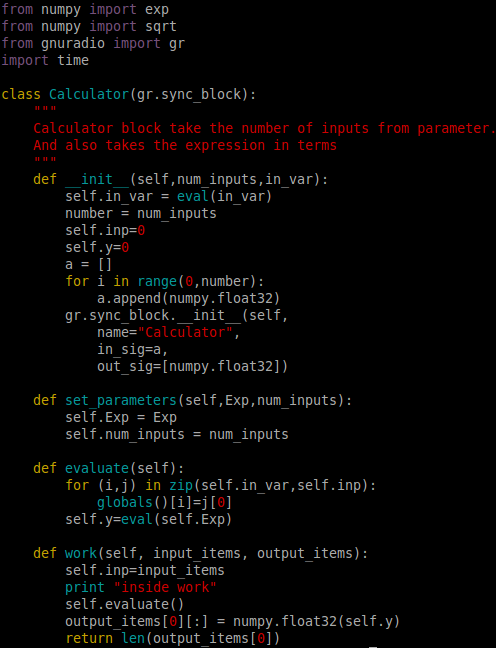
\includegraphics[width=.5\linewidth]{code_screenshot.png}
%            \caption{Flowgraph}
%        \end{minipage}%
%        \begin{minipage}{.5\textwidth}
%            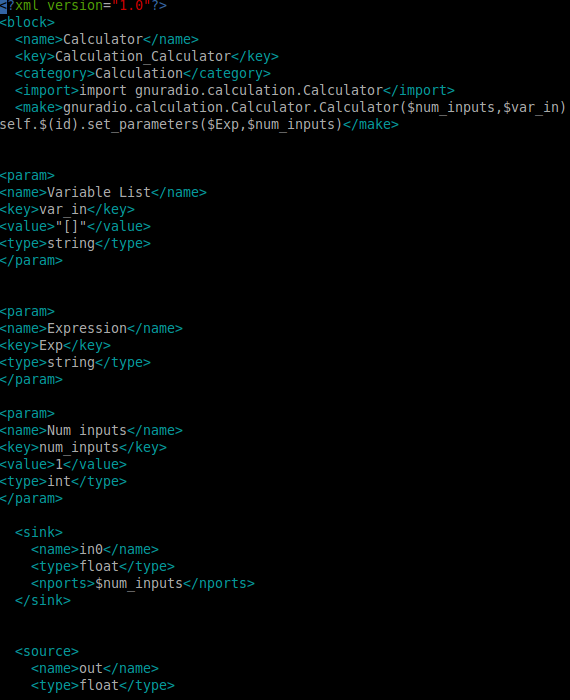
\includegraphics[width=.5\linewidth]{xml_file.png}
%            \caption{Output Plot}
%        \end{minipage}
%    \end{figure}

\end{frame}

\begin{frame}
\frametitle{Work Flow}
\vspace{-0.14in}
\begin{figure}
\centering
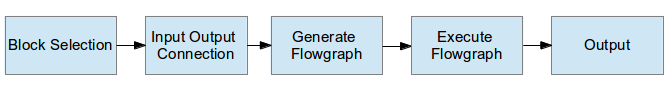
\includegraphics[height=2.8cm, width=10cm]{sandhi_presentation.png}
\end{figure}
\vspace{-0.2in}
\begin{itemize}
\item \textbf{Block:} A functional processing unit with inputs and outputs.
\item \textbf{port:} A single input or output of a block.
\item \textbf{Source:} A producer of data.
\item \textbf{Sink:} A consumer of data.
\end{itemize}
\end{frame}
\begin{frame}
\frametitle{Features}
\begin{itemize}
        \item Applications based on flowgraph can be created in sandhi by connecting blocks as per requirement
        \item In sandhi user can create their own customized blocks using GNU Radio API
        \item It is capable of passing any practical types of data between blocks
        \item User can use scilab script in flowgraph for computation using sciscipy wrapper
        \item Flowgraph with feedback can be create using GRAS
        \item Sandhi provides nice GUI to plot or show data.
        \item User can also change value in real time using slider.
\end{itemize}
\end{frame}
\begin{frame}
        \frametitle{Experiments on sandhi: Data Aquisition}
        \begin{itemize}
	\item Single Board Heater System(SBHS) can controlled using sandhi
	\item Using Python serial library, one can set the fan,heat value to SBHS and receive temperature value from SBHS
        \end{itemize}
\begin{figure}
        \centering
        \begin{minipage}{.5\textwidth}
            \centering
            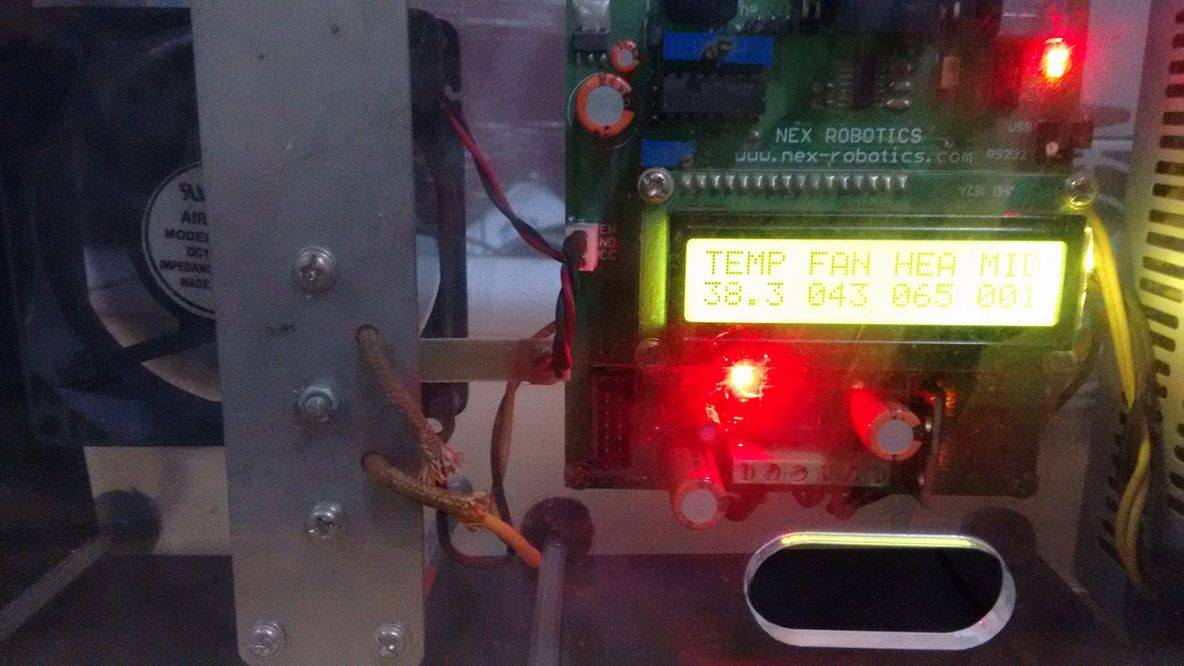
\includegraphics[width=.7\linewidth]{sbhs.jpg}
            \caption{SBHS setup}
        \end{minipage}%
        \begin{minipage}{.5\textwidth}
            \centering
            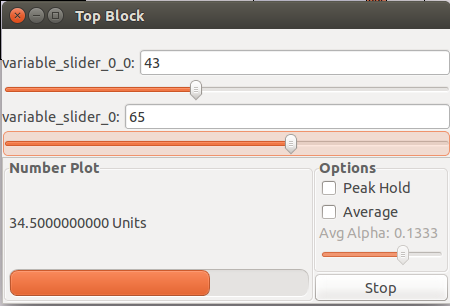
\includegraphics[width=.7\linewidth]{sbhs_img.png}
            \caption{Output Window with slider}
        \end{minipage}
    \end{figure}
%  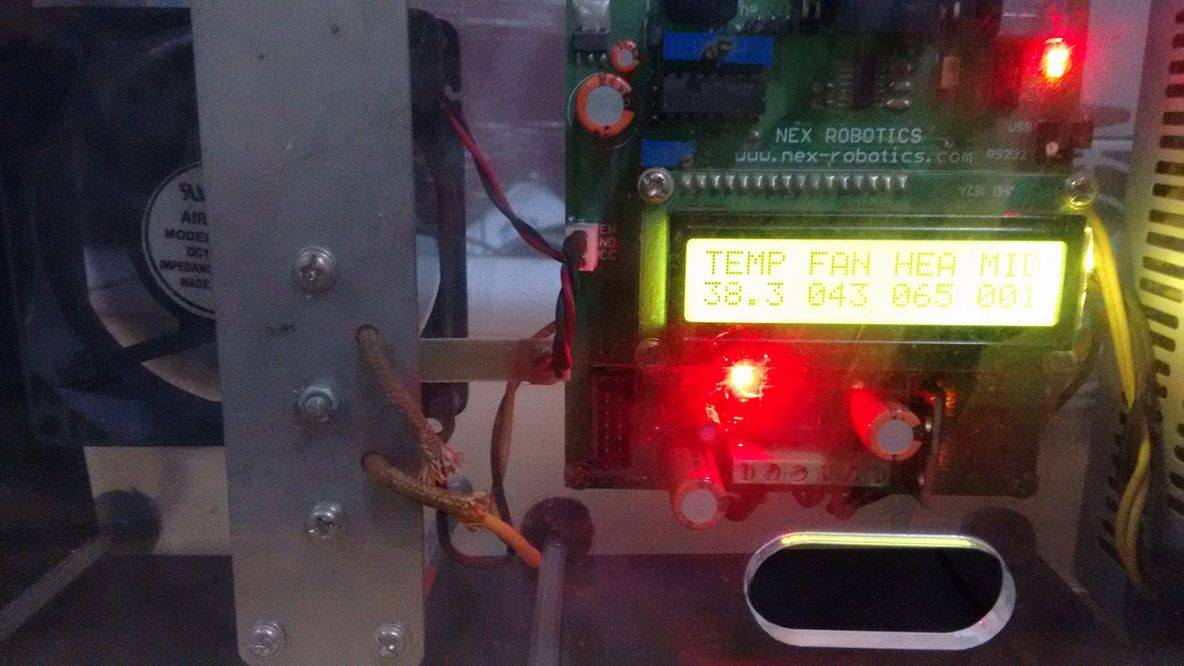
\includegraphics[width=.5\linewidth]{sbhs.jpg}
%  \caption{SBHS showing value of fan, heat and temperature}
%  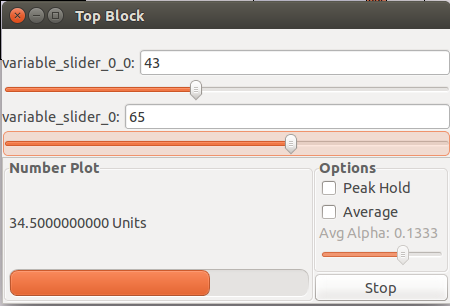
\includegraphics[width=.5\linewidth]{sbhs_img.png}
%  \caption{Output window with slider}
%\begin{figure}
%\subfigure[SBHS showing value of fan, heat and temperature]{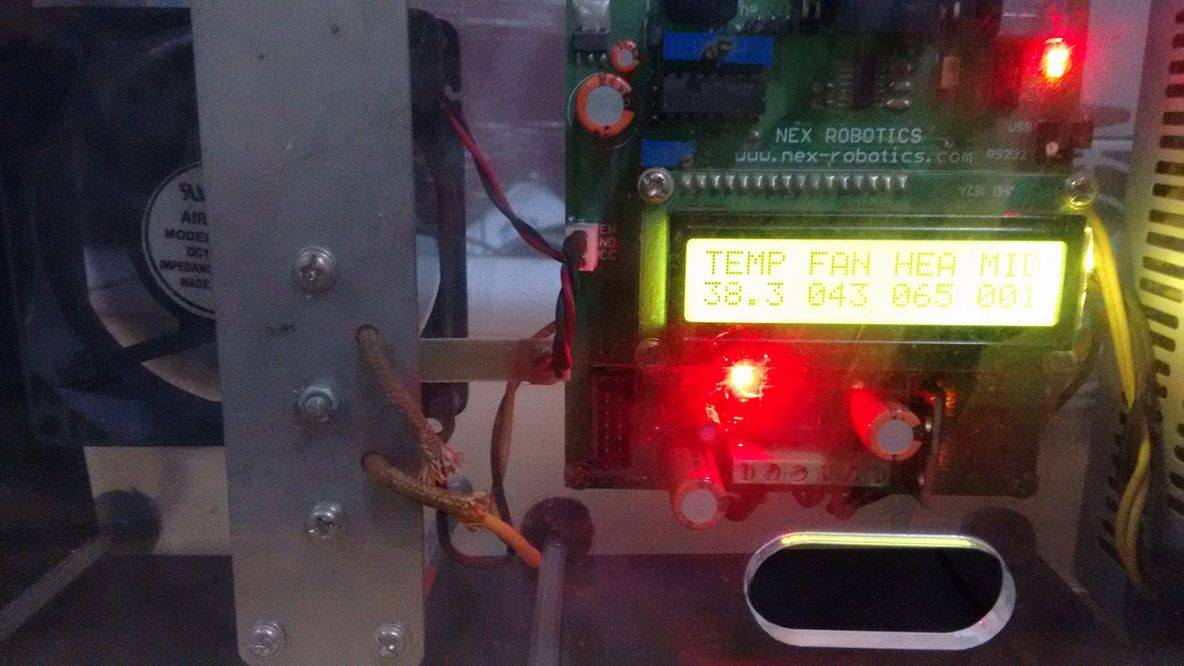
\includegraphics[width=5cm]{sbhs.jpg}}
%\subfigure[Output window with slider]{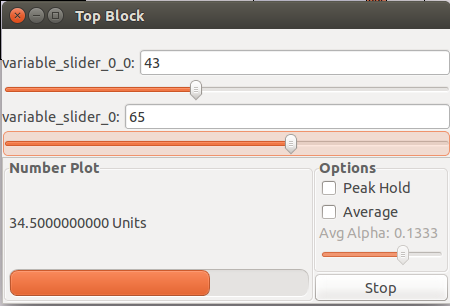
\includegraphics[width=5cm]{sbhs_img.png}}
%\caption{Single Board Heater system running on sandhi}
%\end{figure}
\end{frame}


\begin{frame}
        \frametitle{Experiments on sandhi: step response of transfer function}
        \begin{itemize}
	\item To perform step response the flowgraph is created as follows
	\item Flowgraph uses \textit{Numerator}, \textit{Denomenator}, \textit{Response} and \textit{plot-sink} block
	\item These blocks has been written in Python and response of system is calculated in scilab using sciscipy in Response block
        \end{itemize}
\begin{figure}
        \centering
        \begin{minipage}{.5\textwidth}
            \centering
            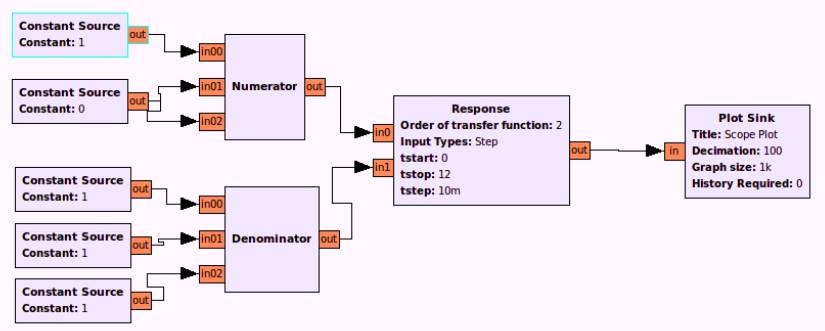
\includegraphics[width=.9\linewidth]{step_resp.png}
            \caption{Flowgraph}
        \end{minipage}%
        \begin{minipage}{.5\textwidth}
            \centering
            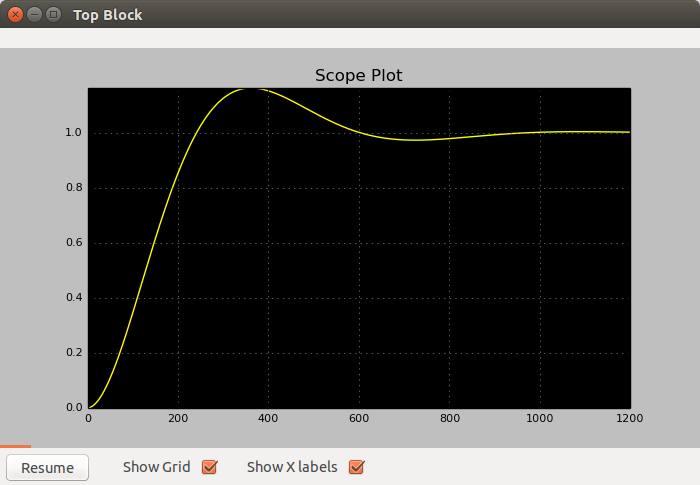
\includegraphics[width=.6\linewidth]{step_out.png}
            \caption{Output Plot}
        \end{minipage}
    \end{figure}
\end{frame}


\begin{frame}
    \frametitle{Architecture}

    \begin{figure}
        \centering
        \begin{minipage}{.5\textwidth}
            \centering
            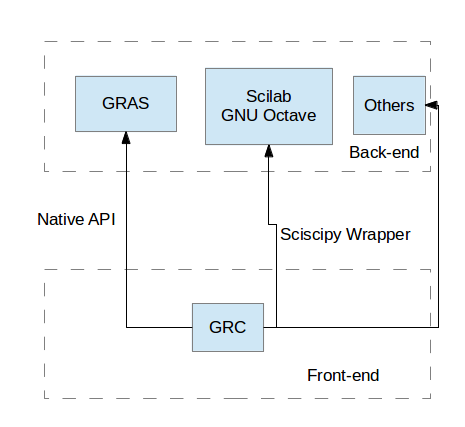
\includegraphics[width=.9\linewidth]{my_img/architecture.png}
            \caption{Sandhi Architecture}
        \end{minipage}%
    \end{figure}

\end{frame}



\begin{frame}
    \frametitle{Closed Loop System}

    \begin{figure}
        \centering
        \begin{minipage}{.5\textwidth}
            \centering
            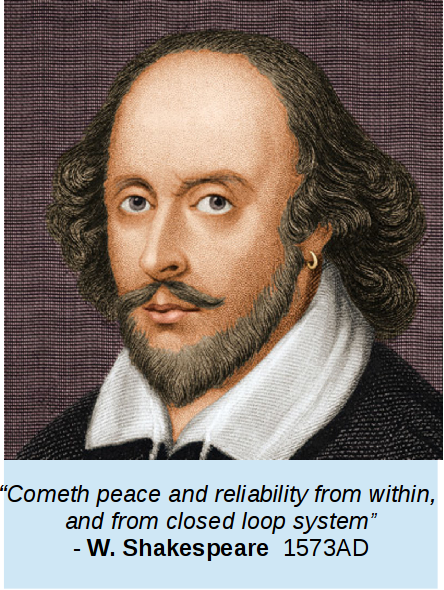
\includegraphics[width=.9\linewidth]{my_img/shaku1.png}
            \caption{Ancient Wisdom}
        \end{minipage}%
    \end{figure}

\end{frame}

\begin{frame}
        \frametitle{GRAS: GNU Radio Advanced Scheduler}
        \begin{itemize}
    \item Written by Josh Blum (josh@joshknows.com)
    \item It is application scheduler
    \item Handles how the blocks(computational entity) should be formed, scheduled
    \item Provides easy API to write our own blocks in Python
    \item Uses Theron, PMC, Apology etc. libraries
        \end{itemize}

\end{frame}

\begin{frame}
    \frametitle{Being Pythonic}

    \begin{figure}
        \centering
        \begin{minipage}{.5\textwidth}
            \centering
            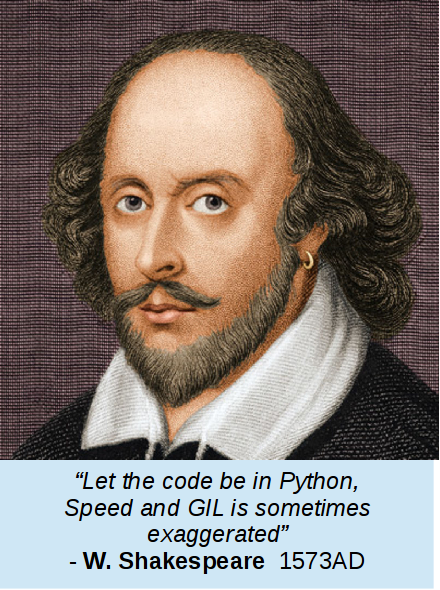
\includegraphics[width=.9\linewidth]{my_img/shaku2.png}
            \caption{Really ancient wisdom}
        \end{minipage}%
    \end{figure}

\end{frame}

\begin{frame}
        \frametitle{Pythonic Sandhi}
    \begin{figure}
        \centering
        \begin{minipage}{.5\textwidth}
            \centering
            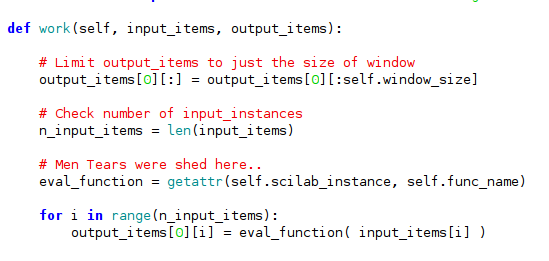
\includegraphics[width=.9\linewidth]{my_img/wf_code_snipped.png}
            \caption{Work Function Code snippet}
        \end{minipage}%
    \end{figure}

\end{frame}


\begin{frame}
\frametitle{Ongoing work}
\begin{itemize}
\item Migrating virtual lab experiments from LABview to Sandhi
\item Improving GUI of Sandhi
\item Addition of features similar to LabView
\item Improving performance of experiments
\item Migration of WX blocks to QT
\item Testing of existing blocks
\item Method to pass Array between blocks
\item Data Aquisition using NI DAQs
\item Control of sampling rate
\item Automatic code generation of blocks
\end{itemize}
\end{frame}

\begin{frame}
\frametitle{Contact Us}
\begin{itemize}
 \item If you are interested to contribute please write to us at {\color{blue} contact-sandhi@fossee.in }
 \item Go through our website {\color{blue} sandhi.fossee.in }
 \item You can post your queries on Forums at {\color{blue} forums.fossee.in }
\end{itemize}
\end{frame}

\begin{frame}
\begin{center}
    \large {\textbf{THANK YOU}}
\end{center}
\end{frame}

\end{document}
